\chapter{Java Server Pages}
Die serverseitige Programmierung wird durch \acrshort{jsp}s realisiert. Dadurch ergeben sich zahlreiche Vorteile, wie das plattformunabhängige Hosting von Websites, Kosten- und Zeitersparnis beim Programmieren und Pflegen des Webauftritts, da Java und dadurch \acrshort{jsp} eine weitverbreitete und dadurch bestens dokumentierte und unterstützte Sprache ist.
\section{Seitenfluss}
In Abbildung \ref{jsp_pflow} ist der Programmfluss der Anwendung schematisch dargestellt. \textit{Start} markiert die \acrshort{jsp}, die beim Starten der Anwendung geladen wird. Die Start\acrshort{jsp} der Anwendung wird in der \textit{web.xml}, die sich im Verzeichnis \textit{"/WebContent/WEB-INF"} befindet, mit der Einstellung in Quellcode \ref{jsp_wf} Zeile 2 definiert.
\begin{lstlisting}[caption={Auswahl der zuerst initialisierten JSP},label=jsp_wf]
  <welcome-file-list>
    <welcome-file>View.jsp</welcome-file>
  </welcome-file-list>
\end{lstlisting}
Von der \textit{View} Seite aus kann man neue Rezepte anlegen (\textit{Edit View}) oder Einträge aus der Übersicht dem Kochbuch hinzufügen, die \textit{Detailansicht} eines Rezeptes aufrufen, von dem aus das Rezept ebenfalls dem Kochbuch hinzugefügt werden kann, oder zur \textit{Kochbuchansicht }wechseln. Von dort aus kann das Kochbuch gelöscht, "gedruckt"\ oder zur \textit{Übersichtsseite (View)} navigiert werden.
Ruft man die \textit{Edit View} auf wird ein neues Rezept in der Session erstellt und man kann entweder zur \textit{Übersichtsseite (View)} zurückkehren oder seine Eingaben überprüfen. Von der \textit{Confirm Ansicht} aus, kann man ein Bild zum Rezept hinzufügen und auf den Server laden oder zur \textit{Equipment} oder \textit{Ingredients} Ansicht wechseln. In diesen können die jeweiligen Optionen dem Rezept hinzugefügt werden und abschließend zum Rezept \textit{(Confirm View)} zurückkehren. Von hier aus kann das Rezept Hinzufügen abgeschlossen werden, indem das Rezept in der Datenbank gespeichert wird. Durch das Sichern \textit{(Save)} wird das Rezept in der Datenbank gespeichert und man kehrt zur \textit{Edit View} zurück, von der aus man (s.o.) neue Rezepte erstellen oder zur Übersichtsseite zurückkehren kann.
\begin{figure}[htbp]
    \centering
    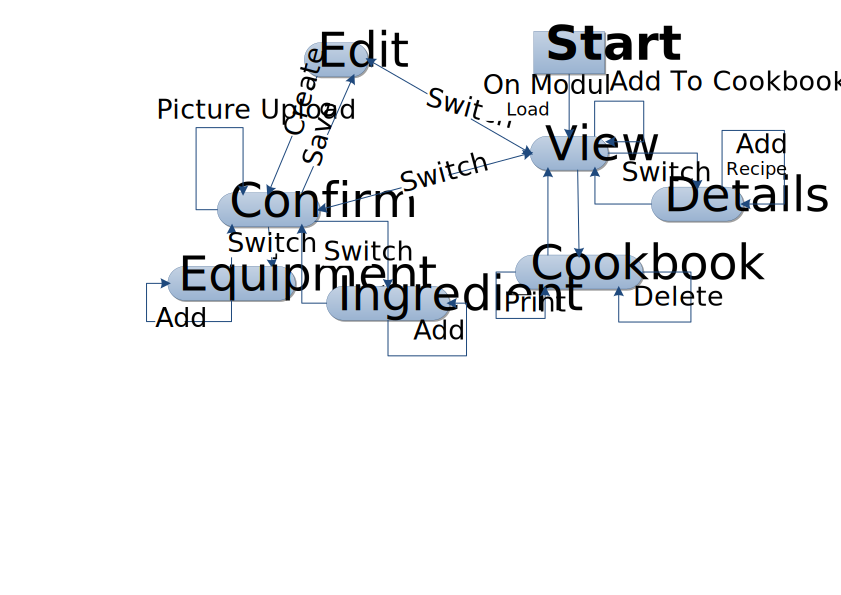
\includegraphics[scale=0.7]{images/programflow.png}
    \caption{Programmfluss der Kochbuchanwendung}
    \label{jsp_pflow}
\end{figure}

\section{Die Edit.jsp Seite}
Die Edit.jsp Seite (s. Quellcode \ref{jsp_edit}) besteht aus einem typischen \acrshort{html}-Gerüst. Teile dieses Gerüsts werden von den in \acrshort{jsp} verfügbaren Direktiven ergänzt. Zu Beginn der Datei werden die Metainformationen zu den Java Bestandteilen aufgelistet.
Ab Zeile 9 beginnt der body des \acrshort{html}-Gerüsts. Durch das \textit{jsp:useBean} in Zeile 10 wird die Klasse \textit{Receipt} (eine jBean) unter dem Variablennamen \textit{receipt} bekannt gemacht und falls unbekannt initialisiert. Mit \textit{scope=\glqq session\grqq} wird der Gültigkeitsbereich der Bean auf die User-Session begrenzt. Defaultwert wäre \textit{page}.
Die \textit{jsp:setProperty} Anweisung setzt alle Attribute der per \textit{jsp:useBean} bekanntgemachten Bean, sofern sie ungleich null sind.  
Darauf folgt ein Formular von Zeile 12-22. Dieses überträgt seine Daten per \textit{POST} und lässt die übertragenen Daten von einem Controller verwalten. Welche Datei beim Aufruf dieses Controllers ausgeführt wird, wird ebenfalls in der \textit{web.xml} Datei definiert.
Das Formular besitzt mehrere Felder. Diese Felder im Textformat sind später über ihren in \textit{name} definierten Index bekannt. Über das Feld des Types \textit{submit} mit dem Index \textit{enterReceipt} werden die Formulardaten mit der \textit{POST}-Methode an den Controller gesendet. Die \textit{Controller.java} Datei, die als Controller aufgerufen wird, prüft zunächst die Parameter des \textit{POST}-Requests. Befindet sich unter dieses Parametern der Index \textit{enterReceipt}, mit dem der Submit des Formulars gesendet wurde, wird die Destination für die Seite, die geladen wird, auf \textit{Confirm.jsp} geändert. Später im Programmfluss des Controllers wird, falls die Destination \textit{Confirm.jsp} ist, überprüft, ob es schon ein Attribut in der Session namens \textit{receipt} gibt. Falls dies nicht der Fall ist, wird ein neues Attribut für das Rezeptobjekt erstellt und mit den Werten aus den Feldern (Titel des Rezepts, Name des Autors, Dauer, Bemerkung, etc.) initialisiert.
Danach befindet sich in Zeile 23 ein Link auf die \textit{View.jsp} Seite, auf der eine Übersicht der bekannten Rezepte angezeigt wird.
\begin{lstlisting}[caption={Die Edit.jsp der Kochbuchanwendung},label=jsp_edit]
<%@ page language="java" contentType="text/html; charset=UTF-8"
    pageEncoding="UTF-8"%>
<!DOCTYPE html PUBLIC "-//W3C//DTD HTML 4.01 Transitional//EN" "http://www.w3.org/TR/html4/loose.dtd">
<html>
<head>
<meta http-equiv="Content-Type" content="text/html; charset=UTF-8">
<title>Rezepteingabe</title>
</head>
<body>
	<jsp:useBean id="receipt" class="model.Receipt" scope="session" />
	<jsp:setProperty property="*" name="receipt"/>
	<form method="POST" action="Controller">
		<table>
			<tr><td>Rezeptname:</td><td><input type="text" name="title"></td></tr>
			<tr><td>Author:</td><td><input type="text" name="author"></td></tr>
			<tr><td>Beschreibung:</td><td><input type="text" name="description"></td></tr>
			<tr><td>Dauer:</td><td><input type="text" name="duration"></td></tr>
			<tr><td>Schwierigkeit:</td><td><input type="text" name="degree"></td></tr>
			<tr><td>Bemerkung:</td><td><input type="text" name="note"></td></tr>
		</table>
		<input type="submit" name="enterReceipt" value="Weiter">
	</form>
	<a href="View.jsp">Zurueck zur Uebersicht</a>
</body>
</html>
\end{lstlisting}

\section{Das verwenden eines Controllers}
Zum verwenden eines Controllers muss dieser der Anwendung bekannt gemacht werden. Dies geschieht, in dem er in der \textit{web.xml} im Verzeichnis \textit{"/WebContent/WEB-INF"} als Servlet eingetragen wird. Ein Beispiel hierfür ist im Quellcode \ref{jsp_ctrl} zu sehen.
\begin{lstlisting}[caption={Beispielkonfiguration für einen Controller},label=jsp_ctrl]
  <servlet>
  	<servlet-name>ControllerServlet</servlet-name>
  	<servlet-class>control.Controller</servlet-class>
  </servlet>
  <servlet-mapping>
  	<servlet-name>ControllerServlet</servlet-name>
  	<url-pattern>/Controller/*</url-pattern>
  </servlet-mapping>
\end{lstlisting}
Die Aufgabe des Controllers ist es den Seitenfluss der Anwendung zu steuern. Er ist Bestandteil des \acrshort{mvc} Patterns und dient dazu die Auswertung der Benutzereingaben und die Logik von der Präsentationsschicht zu trennen. Es ist der Präsentationsschicht egal, was passiert, wenn ein Element geklickt wird. Sie kümmert sich lediglich um die Anzeige der Inhalte der Seite. Der Controller greift dann die ausgelösten Aktionen auf und kümmert sich um die mit den Aktionen verbundene Logik. Dies erhöht die Wartbarkeit von Anwendungen. Vereinfacht die Skalierbarkeit und vermeidet Fehler, da der Programmcode übersichtlicher zu lesen ist. In diesem Fall kümmert sich der Controller hauptsächlich um den Seitenfluss und das dazugehörige Sessionmanagement. Wird ein ausgefülltes Formular gesendet, kümmert sich der Controller um das aufbereiten der nächsten Seite und das verarbeiten der gesendeten Daten.
\section{\acrshort{mvc}-Pattern des Kochbuchs}
Am einfachsten ist die Anwendung des \acrshort{mvc}-Patterns des Kochbuchs zu erkennen, wenn man die Struktur des Projekts (Abb. \ref{jsp_mvc}) betrachtet. Die Struktur lässt durch die Benennung der Pakete direkt die der Model und des Controllers zugehörigen Dateien erkennen. Nimmt man noch die \acrshort{jsp} Dateien im \textit{WebContent} Verzeichnis als Präsentationsschicht hinzu hat man die strukturelle Aufteilung in das \acrshort{mvc}-Pattern komplett.
Der Controller ist, wie oben beschrieben, für den Seitenfluss und das Sessionmanagement zuständig.
Das Model, welches die Daten beinhaltet, enthält in unserem Beispiel die jBeans, die in der Datenbank gespeichert werden. Sie enthalten die Daten, die für die Kochbuchanwendung nötig sind.
Die Präsentationsschicht durch die \acrshort{jsp} Dateien zeichnet sich dadurch aus, dass die JSP Dateien nur die für die Darstellung der Inhalte benötigte Funktionalität beinhalten. So besteht die Anwendung aus drei Hauptfunktionalitäten (Model, View und Controller), wie sie das \acrshort{mvc}-Pattern vorschreibt. Weitere Elemente wie Validierung sind nicht genau definiert und in diesem Fall im \textit{util}-Paket zusammengefasst.
\begin{figure}[htbp]
    \centering
    \includegraphics[scale=1]{images/mvc.png}
    \caption{Strukturansicht des Kochbuch Projekts}
    \label{jsp_mvc}
\end{figure}

